\chapter{Skills Matrix} % Main appendix title

\label{App:matrix} % Change X to a consecutive letter; for referencing this appendix elsewhere, use \ref{AppendixX}

\lhead{Appendix I. \emph{Skills Matrix}} % Change X to a consecutive letter; this is for the header on each page - perhaps a shortened title

This appendix contains three figures.
My skills matrix is displayed in Figure~\ref{fig:matrix}.
The other two figures are graphs that add up the numerical values of the symbols in the matrix (\littlemaster=1, \nomaster=2 and \master=3) to show the cumulative total experience I have had in each LO attainment level (Figure~\ref{fig:cum_LOs}) and how much each course/ work placement contributed to my achievement of the LOs (Figure~\ref{fig:cum_courses}).
Note that:
\begin{itemize}
	\item Asterisks (*) indicate optional courses
	\item Courses to be taken in 2019 are displayed in grey
	\item ``\littlemaster" depicts limited achievement
	\item ``\nomaster" depicts above average achievement
	\item ``\master" depicts full achievement
\end{itemize}

%\begin{figure}
%	\centering
%	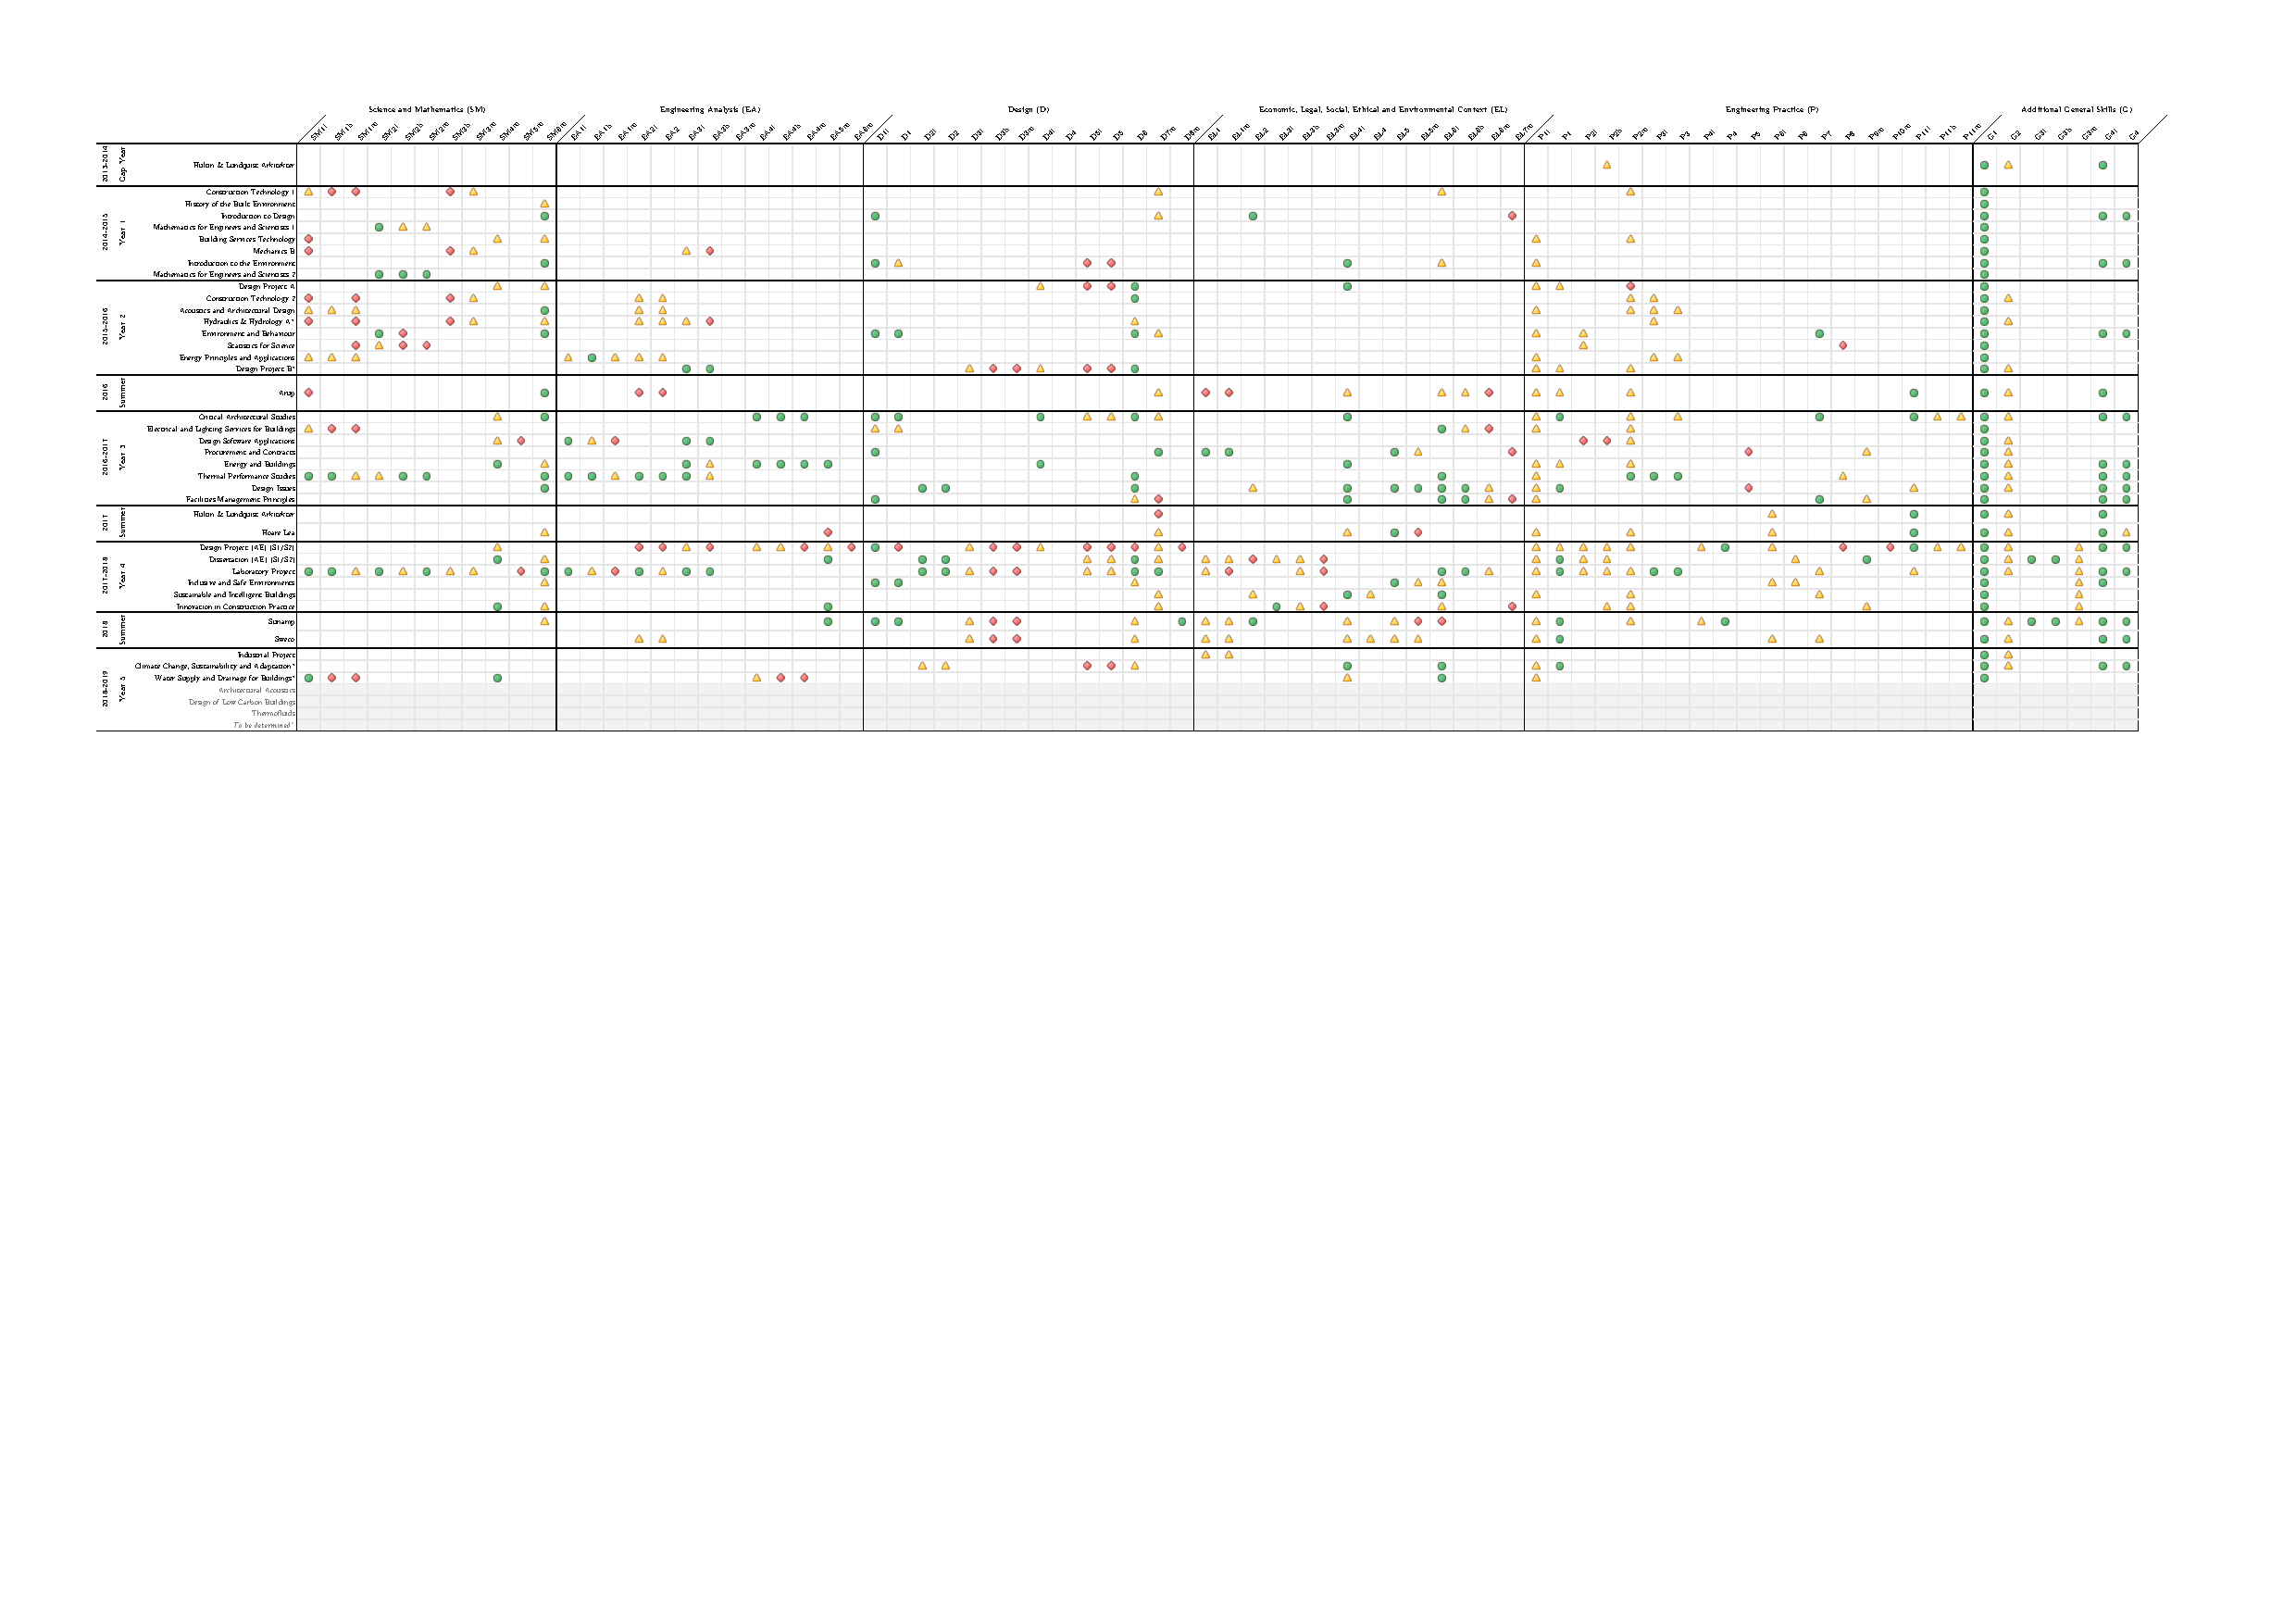
\includegraphics[height=\textheight]{Appendices/Skill-Course-Matrix-small.pdf}
%\end{figure}

\begin{sidewaysfigure}[htbp]
	\centering
	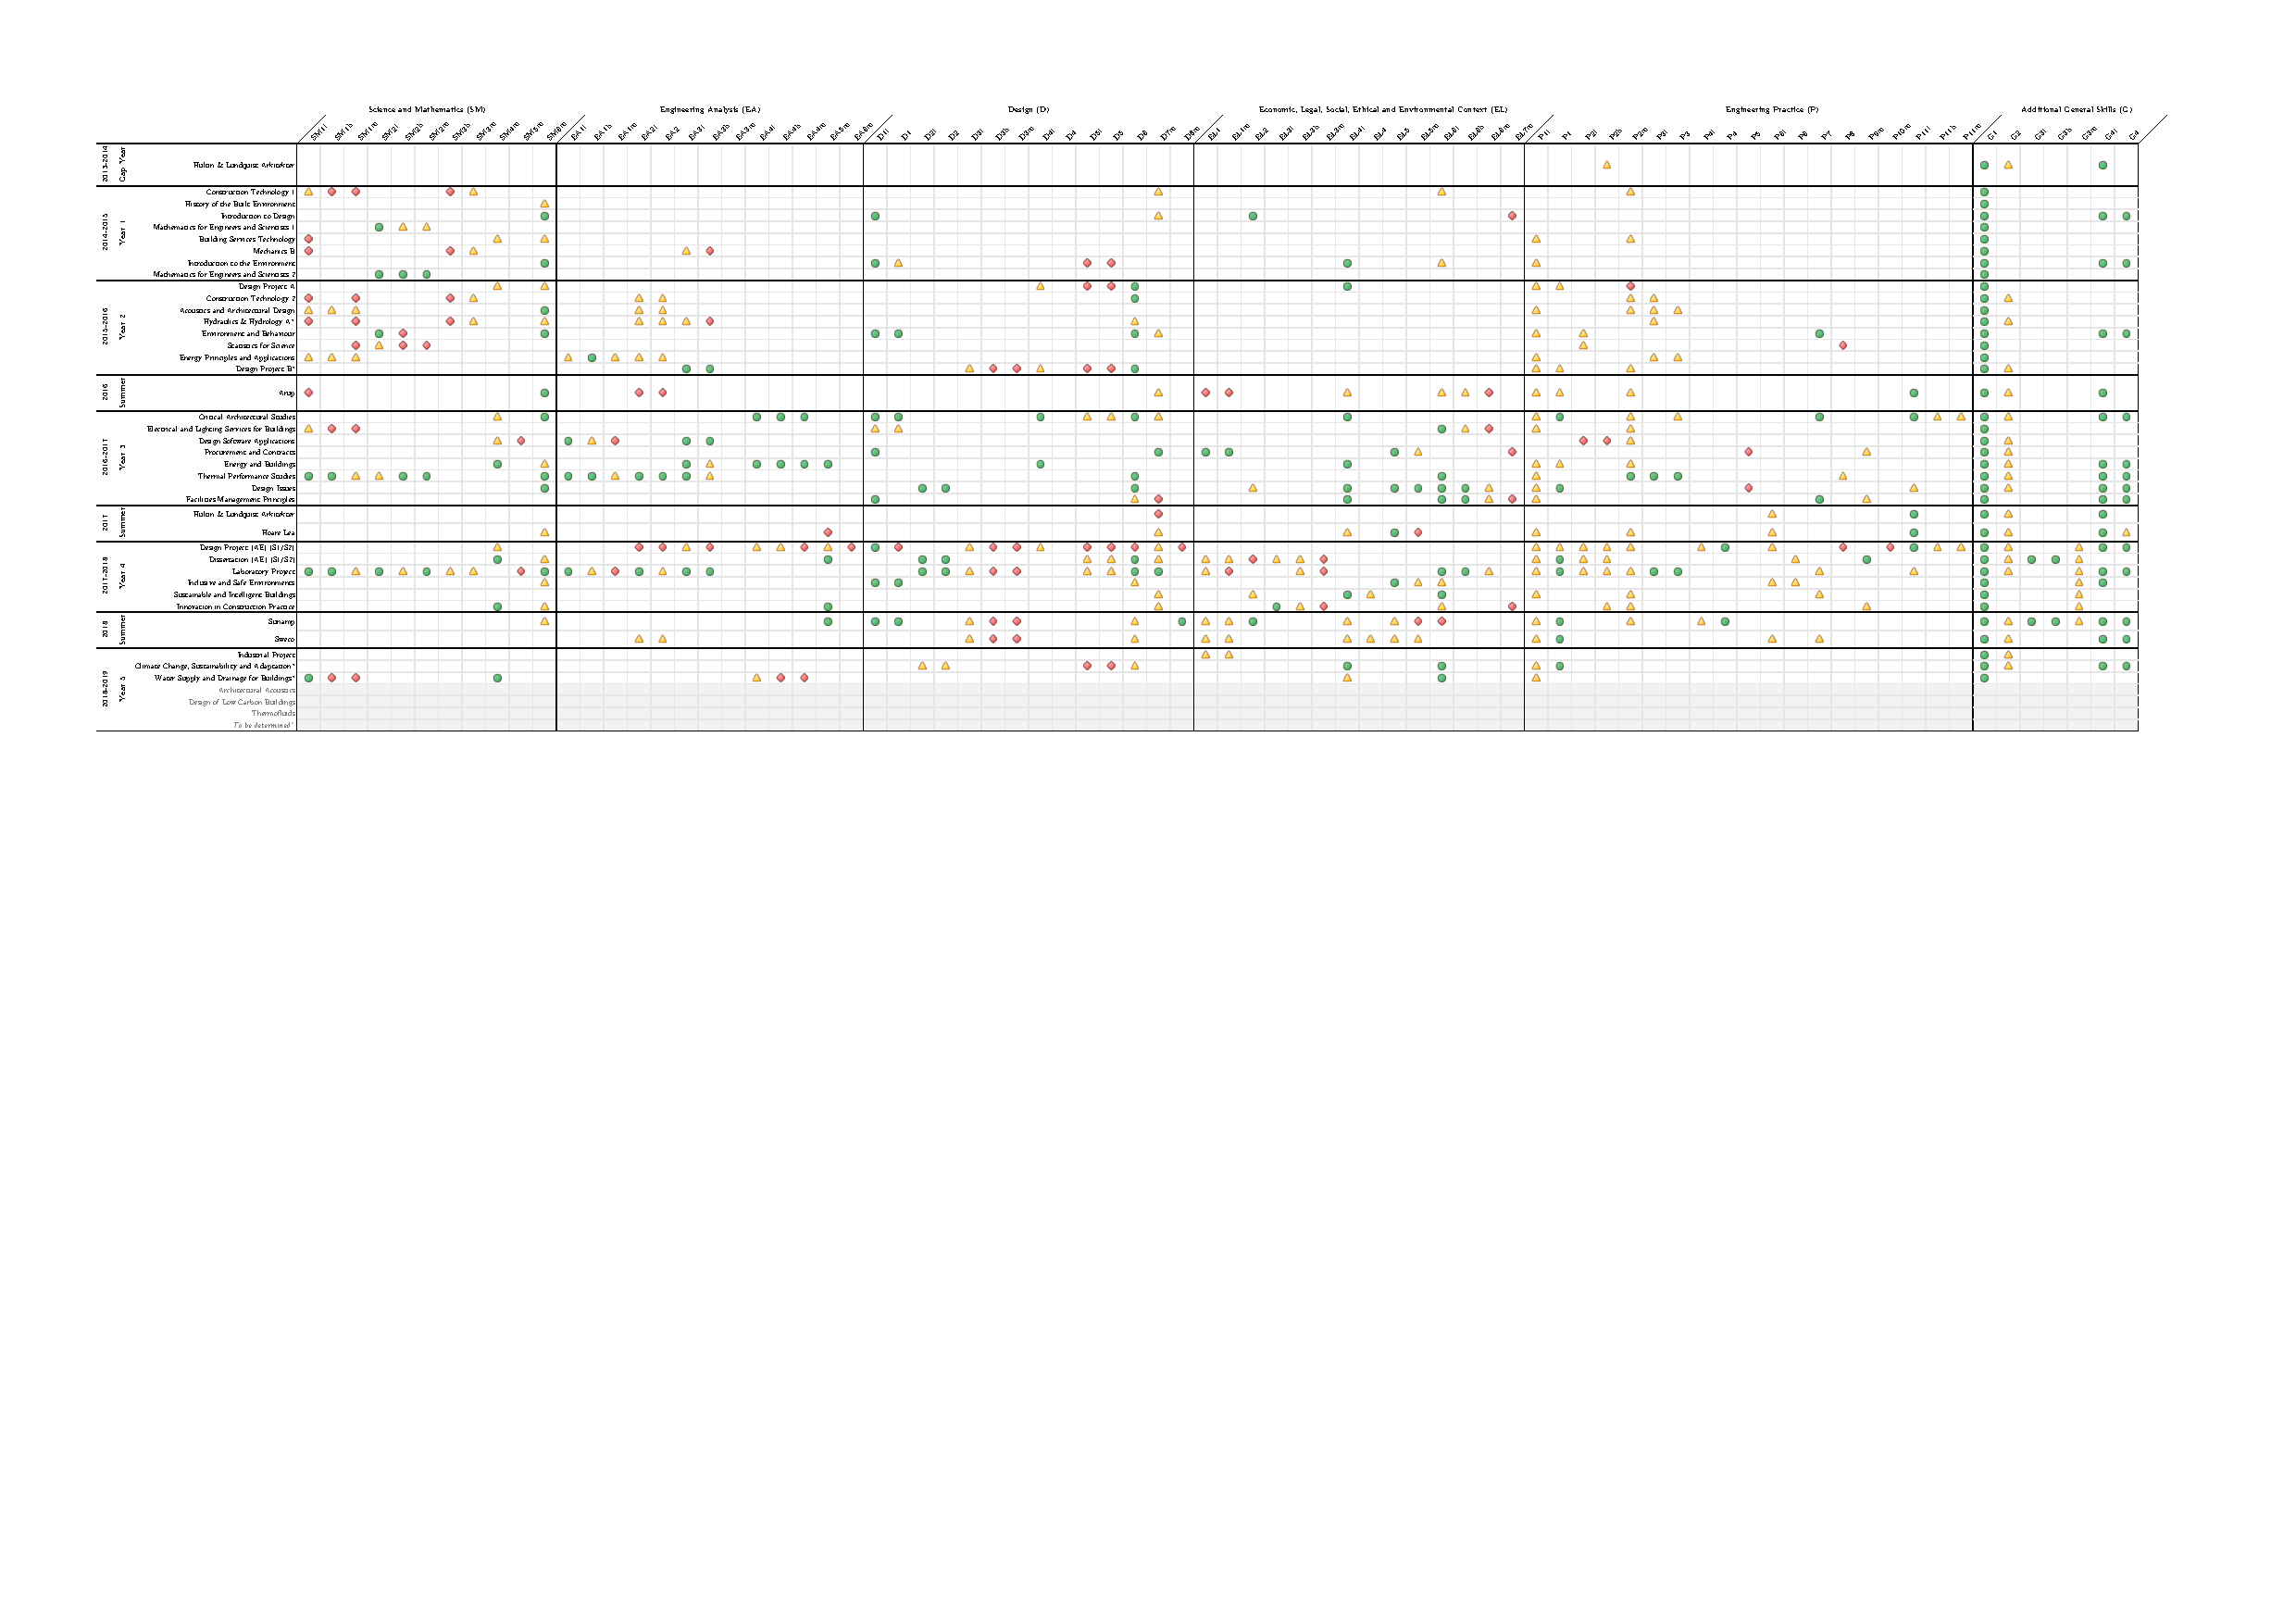
\includegraphics[width=\textwidth]{Appendices/Skill-Course-Matrix-small.pdf}
	\rule{\textwidth}{0.5pt} % use line???
	\caption{Skills matrix.}
	\label{fig:matrix}
\end{sidewaysfigure}


\begin{figure}[htbp]
	\centering
	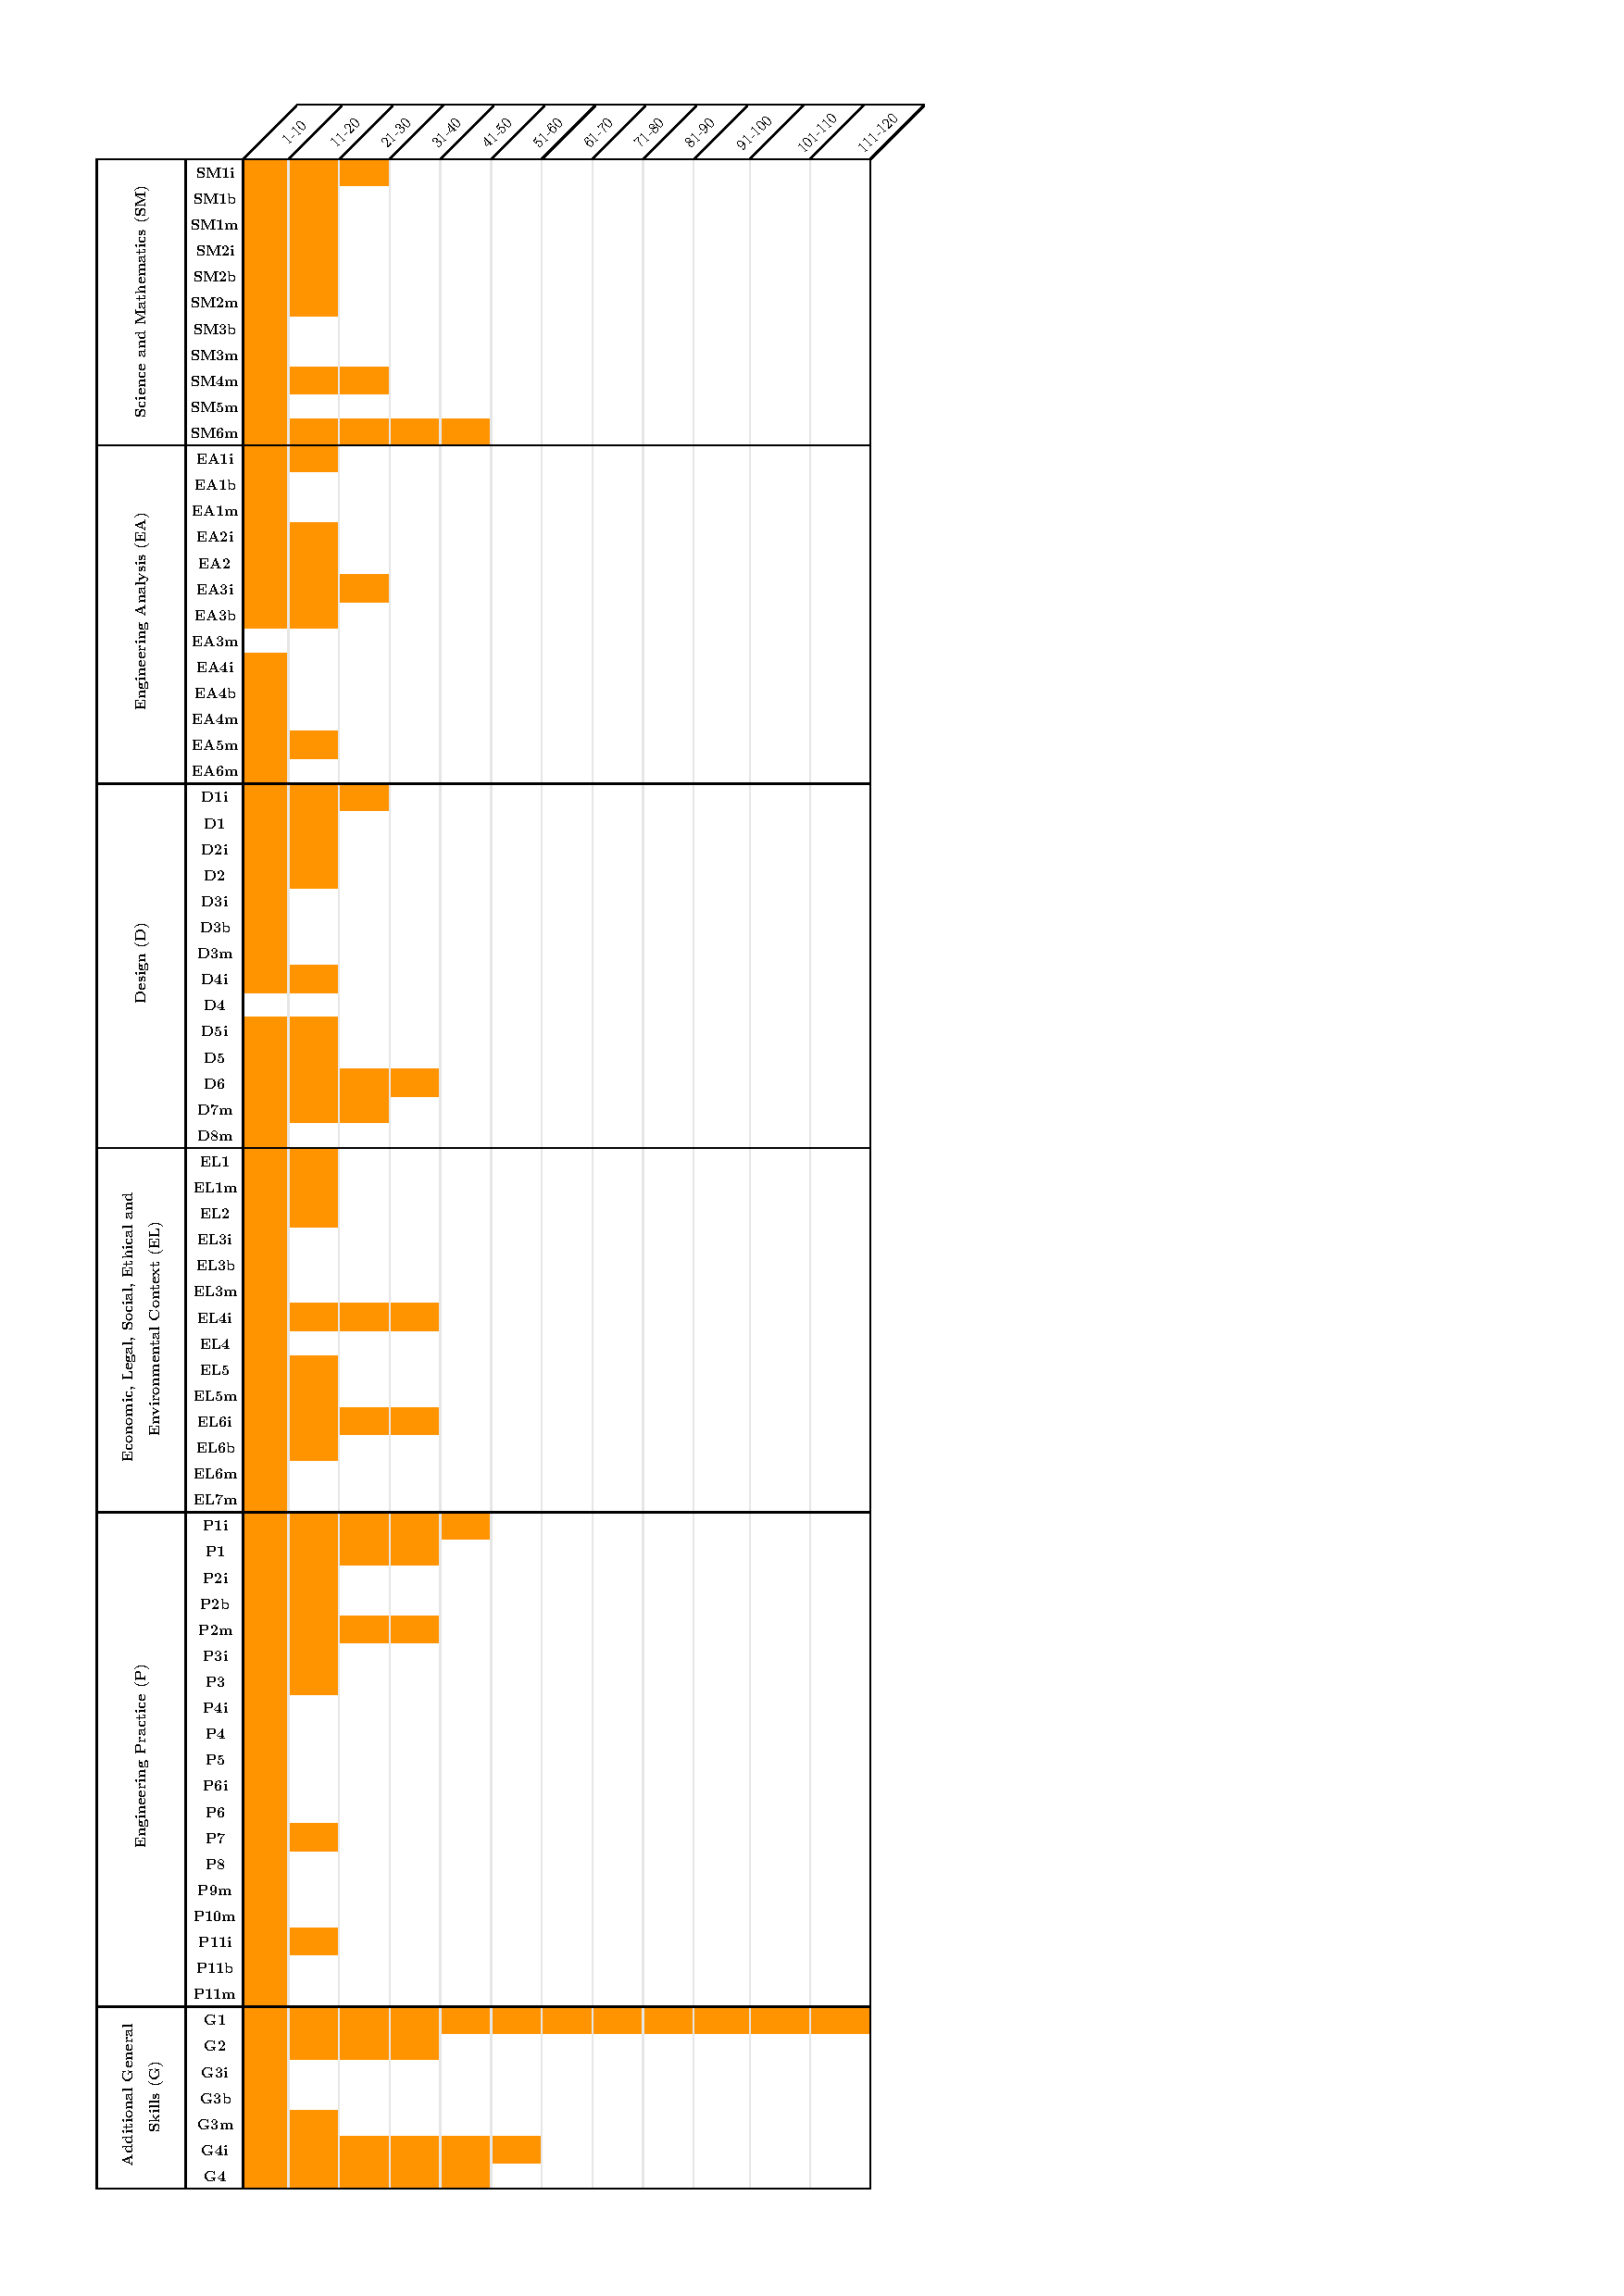
\includegraphics[height=\textheight]{Appendices/Cumulative_LOs_Vertical_Orange_Small.pdf}
	\rule{0.7\textwidth}{0.5pt} % use line???
	\caption{Cumulative total experience in each LO attainment level.}
	\label{fig:cum_LOs}
\end{figure}


\begin{figure}[htbp]
	\centering
	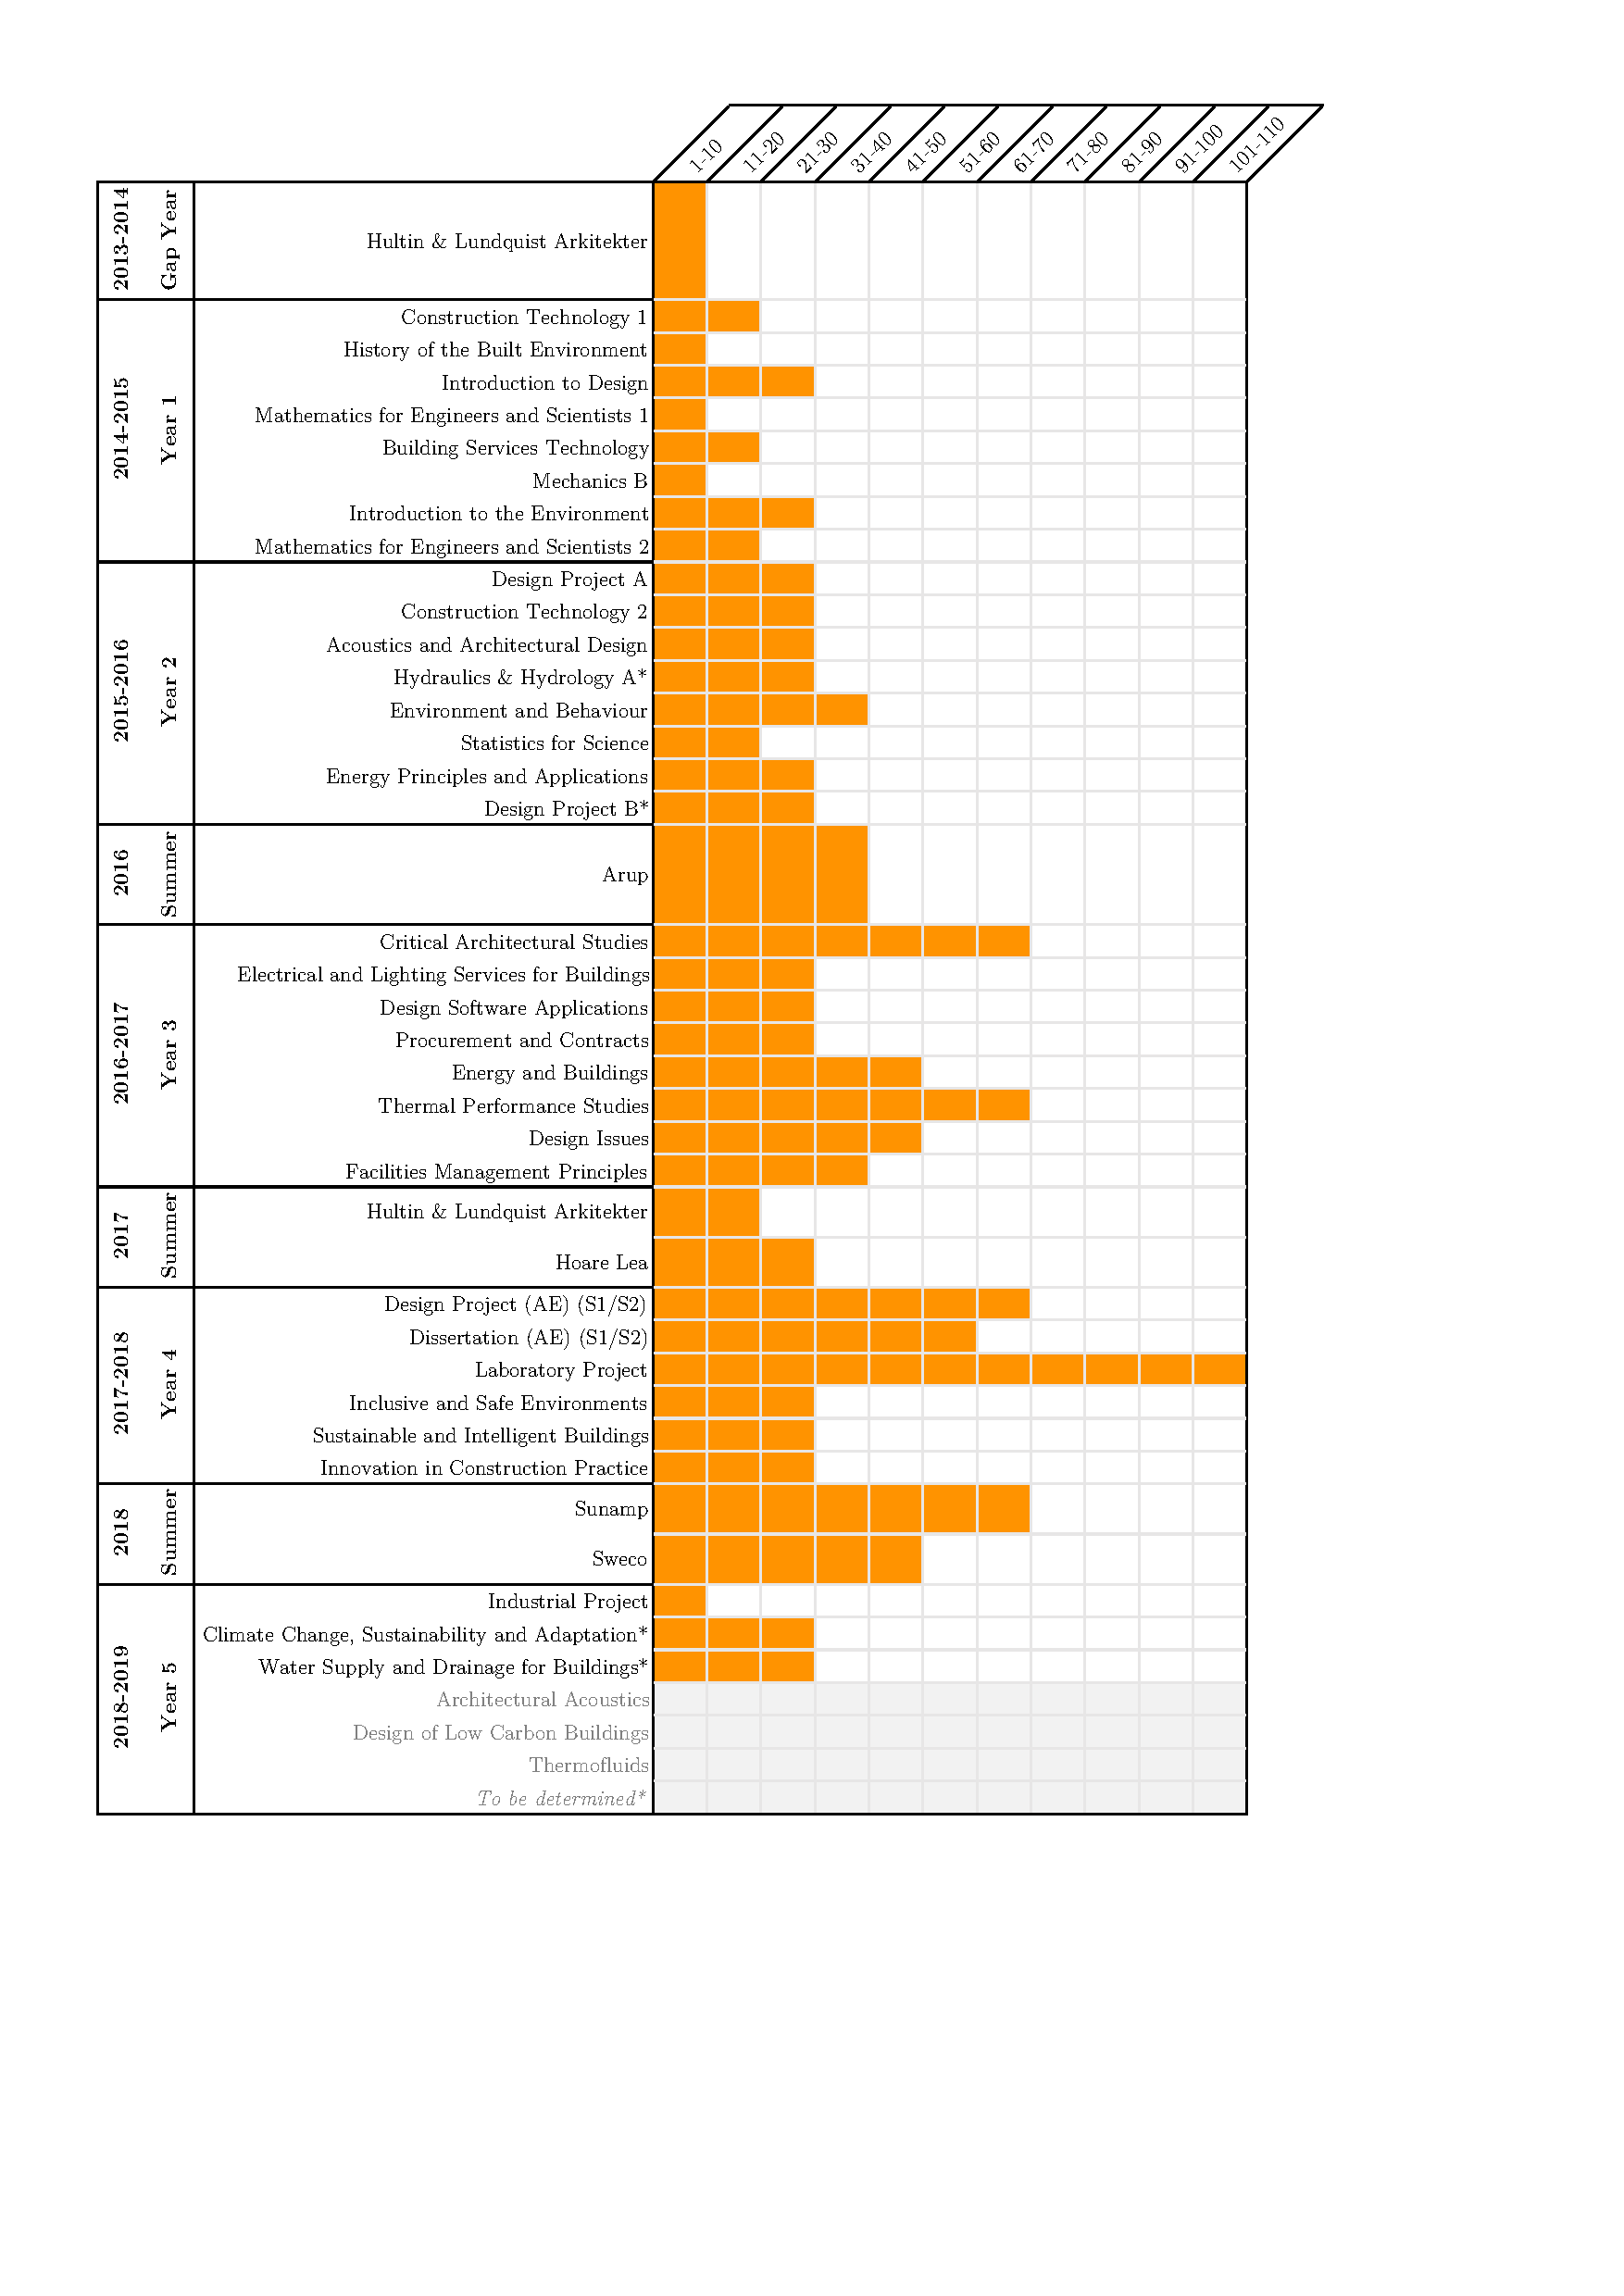
\includegraphics[height=\textheight]{Appendices/Cumulative_Courses_Orange_Small.pdf}
	\rule{\textwidth}{0.5pt} % use line???
	\caption{Cumulative total contribution of every course and work placement to my achievement of the LOs.}
	\label{fig:cum_courses}
\end{figure}